\documentclass{article}

% if you need to pass options to natbib, use, e.g.:
%     \PassOptionsToPackage{numbers, compress}{natbib}
% before loading neurips_2019

% ready for submission
% \usepackage{neurips_2019}

% to compile a preprint version, e.g., for submission to arXiv, add add the
% [preprint] option:
%     \usepackage[preprint]{neurips_2019}
\PassOptionsToPackage{numbers}{natbib}
% to compile a camera-ready version, add the [final] option, e.g.:
\usepackage[final]{neurips_2020}

% to avoid loading the natbib package, add option nonatbib:
%     \usepackage[nonatbib]{neurips_2019}

\usepackage[utf8]{inputenc} % allow utf-8 input
\usepackage[T1]{fontenc}    % use 8-bit T1 fonts
\usepackage{hyperref}       % hyperlinks
\usepackage{url}            % simple URL typesetting
\usepackage{booktabs}       % professional-quality tables
\usepackage{amsfonts}       % blackboard math symbols
\usepackage{nicefrac}       % compact symbols for 1/2, etc.
\usepackage{microtype}      % microtypography
\usepackage{amsfonts}
\usepackage{amsmath}
\usepackage{graphicx}
\graphicspath{ {./images/} }

\usepackage{amsmath,amssymb,bm}
\usepackage{caption}
\captionsetup[figure]{labelfont=small, justification=centering}
\usepackage{subcaption}
\usepackage{mathtools}
\usepackage{lmodern}
\usepackage{siunitx}
\usepackage{booktabs}
\usepackage{etoolbox}

\usepackage[dvipsnames]{xcolor}
\usepackage[hang,flushmargin]{footmisc}
\usepackage{bbm}
\usepackage{pgfplots}
\usetikzlibrary{spy}
\usepgfplotslibrary{external}
\usepgfplotslibrary{fillbetween}
\usetikzlibrary{arrows,automata}
\usepackage{thmtools}
\usepackage{blkarray} 
\usepackage{textcomp}

\usepackage{times}
\usepackage{amsfonts}
\usepackage{amsmath}
\usepackage{latexsym}
\usepackage{color}
\usepackage{graphics}
\usepackage{enumerate}
\usepackage{amstext}
\usepackage{blkarray}
\usepackage{url}
\usepackage{epsfig}
\usepackage{bm}
\usepackage{textcomp}
\usepackage{mathtools}
\usepackage{minted}


\title{Learning to regularize, Application of Neumann Network to the fastMRI dataset}

% The \author macro works with any number of authors. There are two commands
% used to separate the names and addresses of multiple authors: \And and \AND.
%
% Using \And between authors leaves it to LaTeX to determine where to break the
% lines. Using \AND forces a line break at that point. So, if LaTeX puts 3 of 4
% authors names on the first line, and the last on the second line, try using
% \AND instead of \And before the third author name.
\author{%
  Yves Greatti \\
  New York University\\
  % examples of more authors
   \And
    Soham Girish Tamba \\
    New York University\\
}

%% Probability operators and functions
%
% \def \P{\mathrm{P}}
\def \P{\mathrm{P}}
\def \E{\mathrm{E}}
\def \Var{\mathrm{Var}}
\let\var\Var
\def \Cov {\mathrm{Cov}} \let\cov\Cov
\def \MSE {\mathrm{MSE}} \let\mse\MSE
\def \sgn {\mathrm{sgn}}
\def \R {\mathbb{R}}
\def \C {\mathbb{C}}
\def \N {\mathbb{N}}
\def \Z {\mathbb{Z}}
\def \cV {\mathcal{V}}
\def \cS {\mathcal{S}}
\DeclareMathOperator*{\argmin}{arg\,min}
\DeclareMathOperator*{\argmax}{arg\,max}
\newcommand{\red}[1]{\textcolor{red}{#1}}
\newcommand{\blue}[1]{\textcolor{blue}{#1}}
\newcommand{\green}[1]{\textcolor{ForestGreen}{ #1}}
\newcommand{\fuchsia}[1]{\textcolor{RoyalPurple}{ #1}}

%
%% Probability distributions
%
%\def \Bern    {\mathrm{Bern}}
%\def \Binom   {\mathrm{Binom}}
%\def \Exp     {\mathrm{Exp}}
%\def \Geom    {\mathrm{Geom}}
%\def \Norm    {\mathcal{N}}
%\def \Poisson {\mathrm{Poisson}}
%\def \Unif    {\mathrm {U}}
%
\newcommand{\bdb}[1]{\textcolor{red}{#1}}

\newcommand{\ml}[1]{\mathcal{ #1 } }
\newcommand{\wh}[1]{\widehat{ #1 } }
\newcommand{\wt}[1]{\widetilde{ #1 } }
\newcommand{\conj}[1]{\overline{ #1 } }
\newcommand{\rnd}[1]{\tilde{ #1 } }
\newcommand{\rv}[1]{ \rnd{ #1}  }
\newcommand{\rx}{\rnd{ x}  }
\newcommand{\ry}{\rnd{ y}  }
\newcommand{\ra}{\rnd{ a}  }
\newcommand{\rb}{\rnd{ b}  }
\newcommand{\rpc}{\widetilde{ pc}  }

\def \cnd {\, | \,}
\def \Id { I }
\def \J {\mathbf{1}\mathbf{1}^T}

\newcommand{\op}[1]{\operatorname{#1}}
\newcommand{\setdef}[2]{ := \keys{ #1 \; | \; #2 } }
\newcommand{\set}[2]{ \keys{ #1 \; | \; #2 } }
\newcommand{\sign}[1]{\op{sign}\left( #1 \right) }
\newcommand{\trace}[1]{\op{tr}\left( #1 \right) }
\newcommand{\tr}[1]{\op{tr}\left( #1 \right) }
\newcommand{\inv}[1]{\left( #1 \right)^{-1} }
\newcommand{\abs}[1]{\left| #1 \right|}
\newcommand{\sabs}[1]{| #1 |}
\newcommand{\keys}[1]{\left\{ #1 \right\}}
\newcommand{\sqbr}[1]{\left[ #1 \right]}
\newcommand{\sbrac}[1]{ ( #1 ) }
\newcommand{\brac}[1]{\left( #1 \right) }
\newcommand{\bbrac}[1]{\big( #1 \big) }
\newcommand{\Bbrac}[1]{\Big( #1 \Big)}
\newcommand{\BBbrac}[1]{\BIG( #1 \Big)}
\newcommand{\MAT}[1]{\begin{bmatrix} #1 \end{bmatrix}}
\newcommand{\sMAT}[1]{\left(\begin{smallmatrix} #1 \end{smallmatrix}\right)}
\newcommand{\sMATn}[1]{\begin{smallmatrix} #1 \end{smallmatrix}}
\newcommand{\PROD}[2]{\left \langle #1, #2\right \rangle}
\newcommand{\PRODs}[2]{\langle #1, #2 \rangle}
\newcommand{\der}[2]{\frac{\text{d}#2}{\text{d}#1}}
\newcommand{\pder}[2]{\frac{\partial#2}{\partial#1}}
\newcommand{\derTwo}[2]{\frac{\text{d}^2#2}{\text{d}#1^2}}
\newcommand{\ceil}[1]{\lceil #1 \rceil}
\newcommand{\Imag}[1]{\op{Im}\brac{ #1 }}
\newcommand{\Real}[1]{\op{Re}\brac{ #1 }}
\newcommand{\norm}[1]{\left|\left| #1 \right|\right| }
\newcommand{\norms}[1]{ \| #1 \|  }
\newcommand{\normProd}[1]{\left|\left| #1 \right|\right| _{\PROD{\cdot}{\cdot}} }
\newcommand{\normTwo}[1]{\left|\left| #1 \right|\right| _{2} }
\newcommand{\normTwos}[1]{ \| #1  \| _{2} }
\newcommand{\normZero}[1]{\left|\left| #1 \right|\right| _{0} }
\newcommand{\normTV}[1]{\left|\left| #1 \right|\right|  _{ \op{TV}  } }% _{\op{c} \ell_1} }
\newcommand{\normOne}[1]{\left|\left| #1 \right|\right| _{1} }
\newcommand{\normOnes}[1]{\| #1 \| _{1} }
\newcommand{\normOneTwo}[1]{\left|\left| #1 \right|\right| _{1,2} }
\newcommand{\normF}[1]{\left|\left| #1 \right|\right| _{\op{F}} }
\newcommand{\normLTwo}[1]{\left|\left| #1 \right|\right| _{\ml{L}_2} }
\newcommand{\normNuc}[1]{\left|\left| #1 \right|\right| _{\ast} }
\newcommand{\normOp}[1]{\left|\left| #1 \right|\right|  }
\newcommand{\normInf}[1]{\left|\left| #1 \right|\right| _{\infty}  }
\newcommand{\proj}[1]{\mathcal{P}_{#1} \, }
\newcommand{\diff}[1]{ \, \text{d}#1 }
\newcommand{\vc}[1]{\boldsymbol{\vec{#1}}}
\newcommand{\rc}[1]{\boldsymbol{#1}}
\newcommand{\vx}{\vec{x}}
\newcommand{\vy}{\vec{y}}
\newcommand{\vz}{\vec{z}}
\newcommand{\vu}{\vec{u}}
\newcommand{\vv}{\vec{v}}
\newcommand{\vb}{\vec{\beta}}
\newcommand{\va}{\vec{\alpha}}
\newcommand{\vaa}{\vec{a}}
\newcommand{\vbb}{\vec{b}}
\newcommand{\vg}{\vec{g}}
\newcommand{\vw}{\vec{w}}
\newcommand{\vh}{\vec{h}}
\newcommand{\vnu}{\vec{\nu}}
\newcommand{\rvnu}{\vc{\nu}}

\newtheorem{theorem}{Theorem}[section]
% \declaretheorem[style=plain,qed=$\square$]{theorem}
\newtheorem{corollary}[theorem]{Corollary}
\newtheorem{definition}[theorem]{Definition}
\newtheorem{lemma}[theorem]{Lemma}
\newtheorem{remark}[theorem]{Remark}
\newtheorem{algorithm}[theorem]{Algorithm}

% \theoremstyle{definition}
%\newtheorem{example}[proof]{Example}
%\declaretheorem[style=definition,qed=$\triangle$,sibling=definition]{example}
%\declaretheorem[style=definition,qed=$\bigcirc$,sibling=definition]{application}

%
%% Typographic tweaks and miscellaneous
%\newcommand{\sfrac}[2]{\mbox{\small$\displaystyle\frac{#1}{#2}$}}
%\newcommand{\suchthat}{\kern0.1em{:}\kern0.3em}
%\newcommand{\qqquad}{\kern3em}
%\newcommand{\cond}{\,|\,}
%\def\Matlab{\textsc{Matlab}}
%\newcommand{\displayskip}[1]{\abovedisplayskip #1\belowdisplayskip #1}
%\newcommand{\term}[1]{\emph{#1}}
%\renewcommand{\implies}{\;\Rightarrow\;}

% My macros

\def\Kset{\mathbb{K}}
\def\Nset{\mathbb{N}}
\def\Qset{\mathbb{Q}}
\def\Rset{\mathbb{R}}
\def\Sset{\mathbb{S}}
\def\Zset{\mathbb{Z}}
\def\squareforqed{\hbox{\rlap{$\sqcap$}$\sqcup$}}
\def\qed{\ifmmode\squareforqed\else{\unskip\nobreak\hfil
\penalty50\hskip1em\null\nobreak\hfil\squareforqed
\parfillskip=0pt\finalhyphendemerits=0\endgraf}\fi}

%\DeclareMathOperator*{\E}{\rm E}
%\DeclareMathOperator*{\argmax}{\rm argmax}
%\DeclareMathOperator*{\argmin}{\rm argmin}
%\DeclareMathOperator{\sgn}{sign}
\DeclareMathOperator{\supp}{supp}
\DeclareMathOperator{\last}{last}
%\DeclareMathOperator{\sign}{\sgn}
\DeclareMathOperator{\diag}{diag}
\providecommand{\abs}[1]{\lvert#1\rvert}
\providecommand{\norm}[1]{\lVert#1\rVert}
\def\vcdim{\textnormal{VCdim}}
\DeclareMathOperator*{\B}{\textbf{B}}

%\DeclarePairedDelimiter\ceil{\lceil}{\rceil}
%\DeclarePairedDelimiter\floor{\lfloor}{\rfloor}

\newcommand{\cX}{{\mathcal X}}
\newcommand{\cY}{{\mathcal Y}}
\newcommand{\cA}{{\mathcal A}}
\newcommand{\ignore}[1]{}
\newcommand{\bi}{\begin{itemize}}
\newcommand{\ei}{\end{itemize}}
\newcommand{\be}{\begin{enumerate}}
\newcommand{\ee}{\end{enumerate}}
\newcommand{\bd}{\begin{description}}
\newcommand{\ed}{\end{description}}
\newcommand{\h}{\widehat}
\newcommand{\e}{\epsilon}
\newcommand{\mat}[1]{{\mathbf #1}}
%\newcommand{\R}{\mat{R}}
\newcommand{\0}{\mat{0}}
\newcommand{\M}{\mat{M}}

\newcommand{\D}{\mat{D}}
\renewcommand{\r}{\mat{r}}
\newcommand{\x}{\mat{x}}
\renewcommand{\u}{\mat{u}}
\renewcommand{\v}{\mat{v}}
\newcommand{\w}{\mat{w}}
\renewcommand{\H}{\text{0}}
\newcommand{\T}{\text{1}}
%\newcommand{\set}[1]{\{#1\}}
\newcommand{\xxi}{{\boldsymbol \xi}}
\newcommand{\ssigma}{{\boldsymbol \sigma}}
\newcommand{\Alpha}{{\boldsymbol \alpha}}
\newcommand{\tts}{\tt \small}
\newcommand{\hint}{\emph{hint}}
\newcommand{\matr}[1]{\bm{#1}}     % ISO complying version
\newcommand{\vect}[1]{\bm{#1}} % vectors

%\newcommand{\Var}{\mathrm{Var}}
%\newcommand{\Cov}{\mathrm{Cov}}

% New commands
\newcommand{\SP}{\mathbf{S}_{+}^n}
\newcommand{\Proj}{\mathcal{P}_{\mathcal{S}}}
\DeclarePairedDelimiterX{\inp}[2]{\langle}{\rangle}{#1, #2}


\begin{document}

\maketitle

\begin{abstract}
 Recent progress in Machine Learning and Data science has seen the development of efficient Neural Networks architecture to solve inverse-problems. Neural networks have surpassed more traditional approaches in 
  many natural sciences, medicine and life sciences, challenging applications.
 Our goal in this work has been first to perform a quick survey of data-driven inverse problem methodologies, followed by an understanding of the key ideas at the core of a Neumann Network and its implementation
 and application to the task of image reconstruction using the fastMRI dataset, a very-large collection of  undersampled Magnetic Resonance Imaging (MRI) measurements. 
  \end{abstract}
  
 \section{Introduction}
\label{Introduction}

In term of operator, an inverse problem is formalized as solving an operator equation
\begin{equation}
	\matr{Y} = \mathcal{A} (\beta_{\text{true}}) + \epsilon \label{eq:1}
\end{equation}
where $\mathcal{A}$ is a forward operator from the model parameter space $\matr{X}$ to the data space $\matr{Y}$,  $\beta_{\text{true}}$ the ground truth image and $\epsilon$ a random variable modeling the observation noise.
 The MRI (Magnetic Resonance Imaging) image reconstruction problem is an inverse problem, the forward operator is a discrete sampling operator concatenated with the Fourier transform.
 To eliminate image artifacts due to patient movements, an MRI machine acquires less data to reduce the scan time.
For the fastMRI image reconstruction challenge, the undersampling consists  in masking k-space lines from a fully-sampled acquisition.
A difficulty in solving  \eqref{eq:1}, is that the solution is sensitive to variations in the data, which is referred to ill-posedness. The notion of  ill-posedness is attributed to Hadamard, who defined that, by contrast, a well-posed problem
has three distinct properties: (1) it has a solution, that is unique (2), and that depends continuously on the data (3). Another way of describing  ill-posedness is to understand the operator  $\mathcal{A}$ and when it is linear , look at its singular
value decomposition. The decay of the spectral spectrum $\sigma_k, k \in \mathcal{N}$ of  $\mathcal{A}$ is strongly related to the ill-posedness: faster decay implies a more ill-posed problem. 
 	
	\begin{figure}[H]
		\centering
		\captionsetup{justification=centering}
		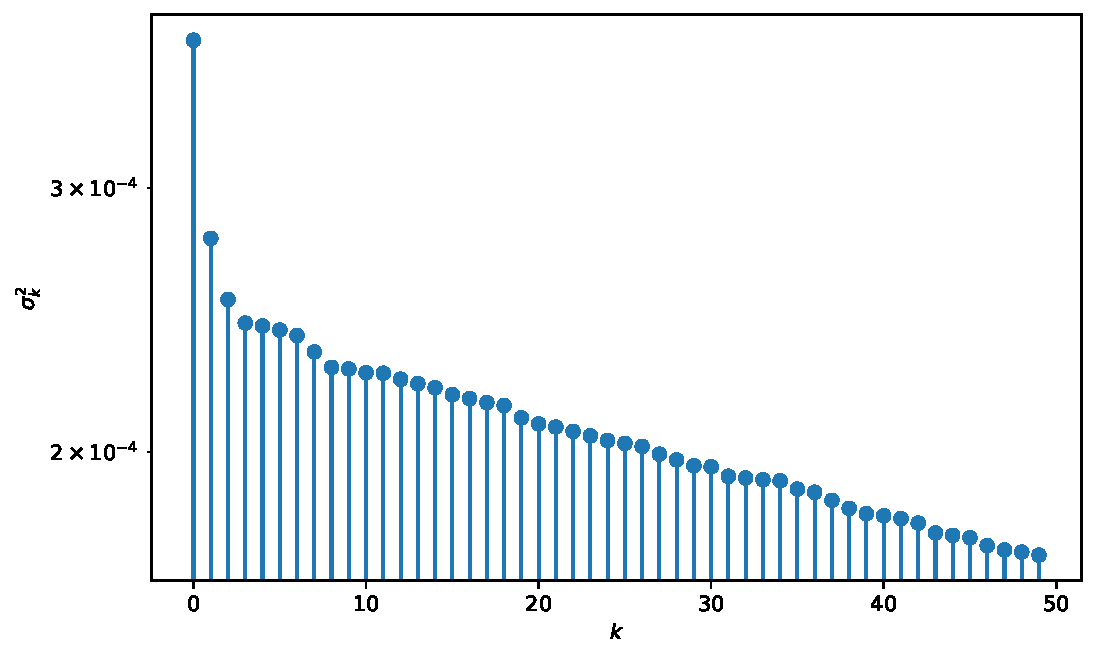
\includegraphics[width=200pt]{variance_plot_log.pdf}
		\caption{$50$ first singular value of the k-space of an image from the fastMRI dataset after undersampling.}
	\end{figure}
The problem defined in \eqref{eq:1}, can be formulated as an ordinary least squares problem (OLS) , given a set of training images $\{\vect{y_1}, \vect{y_2}, \ldots, \vect{y_n}\}$, and an operator $\mathcal{A}$, we want to compute the estimates 
$\vect{\beta}$ which satisfy:
$$
\hat{\vect{\beta}}  =  \argmin_{\beta} \| \vect{y} -\mathcal{A} \vect{\beta} \|_2^2
$$
The aim of regularization theory is to provide a regularizer $r(\cdot)$ which pushes the estimate $\vect{\beta}$ to $\vect{\beta}_{\text{true}}$. We now set the inverse problem as:
$$
\hat{\vect{\beta}}  =  \argmin_{\beta} \frac{1}{2} \| \vect{y} -\mathcal{A} \vect{\beta} \|_2^2 + r(\vect{\beta})
$$
The regularization operator $r(\cdot)$, is a denoising encoder and one approach to solve these inverse problems is to learn $r(\cdot)$. 
 
\section{Theory}
\label{Theory}

The core idea of a Neumann network, it is to use a denoising autoencoder as a proximal operator in an iterative scheme.
The estimated reconstructed image is given by:
\begin{equation}
\op{prox}_{r}\brac{\vect{\beta}} := \arg \min_{\vect{\beta}} r\brac{\vect{\beta}}+ \frac{1}{2} \normTwo{\vect{y}-\matr{X}\vect{\beta}}^2  \label{eq:2}
\end{equation}

Assuming that $r\brac{\vect{\beta}} = \frac{1}{2} \vect{\beta}^T \vect{R} \vect{\beta}$ then taking the gradient of the \eqref{eq:2}, leads to the optimal solution $\vect{\beta}^{\ast}$
\begin{align*}
	(\matr{X}^T \matr{X} + \matr{R}) \matr{\beta}^* &=	\matr{X}^T \vect{y} \\
	\matr{\beta}^* 			&= (\matr{X}^T \matr{X} + \matr{R})^{-1} \matr{X}^T \vect{y} \\
\end{align*}
Using a well-established  result,  for any matrix, $ p \times p \, \matr{A}$, the Neumann series, $\sum_{k=0}^\infty \matr{A}^k$, converges to the inverse of $\matr{I} - \matr{A}$,
assuming $\|\matr{A}\|_{l_i} < 1$ where $l_i$ is an operator norm. We are now in position to replace the inversion defined in  \eqref{eq:2}, by a finite sum of power of $\matr{A}$:
\begin{align*}
	(\matr{I} - \matr{A})^{-1}	&= \sum_{k=0}^{\infty} \matr{A}^k = \matr{I} + \matr{A} + \matr{A}^2 + \matr{A}^3 + \cdots \\ 
	\matr{B}^{-1}			&= \eta  \sum_{k=0}^{\infty}  (\matr{I} - \eta \matr{B})^k \text{~ ancillary result} \\	
	\matr{\beta}^*			&=  \sum_{j=0}^{\infty} (\matr{I} - \eta \matr{X}^T \matr{X} -\eta \matr{R})^j (\eta \matr{X}^T \vect{y}) \\
	\hat{\matr{\beta}}(\vect{y})  &:=  \sum_{j=0}^{B} \bigg([ \matr{I} - \eta \matr{X}^T \matr{X} ](\cdot) -\eta \matr{R}(\cdot) \bigg)^j (\eta \matr{X}^T \vect{y}) \\	
\end{align*}
The last equation has a natural recursive form which is easily interpretable as a deep learning architecture:
\begin{align*}
	\tilde{\vect{\beta}}^{(j)} 		&:=	\bigg( \matr{I} - \eta \matr{X}^T \matr{X} \bigg) \tilde{\vect{\beta}}^{(j-1)} - \eta R(\tilde{\vect{\beta}}^{(j-1)}), j=1, \cdots , B \\
	\tilde{\vect{\beta}}(\vect{y})	&:=   \sum_{j=0}^{B} \tilde{\vect{\beta}}^{(j)} \\
\end{align*}
	\begin{figure}[H]
		\centering
		\captionsetup{justification=centering}
		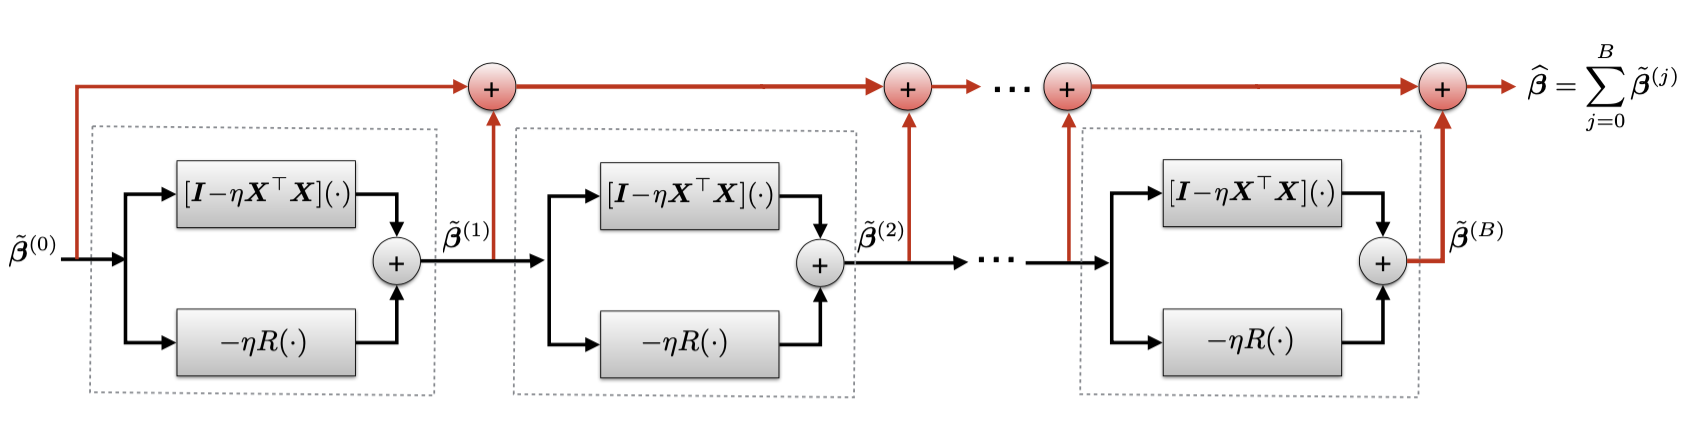
\includegraphics[width=400pt]{nn_architecture}
		\caption{Neumann Network Architecture}
	\end{figure}
One interesting lemma established by Gilton et Al, is that the finite sum $\sum_{j=0}^{B} \tilde{\vect{\beta}}^{(j)} $ provides indeed an estimate for the reconstructed image $\tilde{\vect{\beta}}(\vect{y})$  approximatvely equal to the optimal reconstruction  $\vect{\beta}^{\ast}$, almost \emph{independently} of the number of iterations, which is a result we recovered through our experiments.

Assuming that the autoencoder is linear with the input 
$$
	\vect{R}(\matr{\beta}) = \vect{R} \matr{\beta} = -c_{\eta,B} ( \matr{I} - \matr{X}^T \matr{X}) 
	\matr{U} (\matr{U}^T   \matr{X}^T \matr{X}  \matr{U})^{-1} \matr{U}^T   \matr{X}^T \matr{X} 
$$ where $\tilde{\vect{\beta}}^{(0)} = \eta \matr{X}^T \vect{y}, \vect{y} = \matr{X} \vect{\beta}^{\ast}$

then
\begin{align*}
	\tilde{\vect{\beta}}^{(j)}			&=  a_j \matr{X}^T \matr{X} \vect{\beta}^* + b_j (\matr{I} - \matr{X}^T \matr{X} ) \vect{\beta}^* \\
		&\text{ where } \sum_j a_j \approx 1 \text{ and }  \sum_j b_j \approx 1  \\
	\hat{\vect{\beta}}(\vect{y})	&= \sum_{j=0}^B \tilde{\vect{\beta}}^{(j)} \\
						&\approx \matr{X}^T \matr{X}  \vect{\beta}^* + (\matr{I} - \matr{X}^T \matr{X} ) \vect{\beta}^* =   \vect{\beta}^* \\
\end{align*}


\section{MRI Experiments}
\label{MRIExperiments}

PLEASE START HERE DESCRIPTION OF FAST MRI 


  
%\bibliographystyle{plainnat}
%\bibliography{references}
\end{document}

